\documentclass[12pt,a4paper]{article}

% Fonts and encoding
\usepackage[T1]{fontenc}
\usepackage[utf8]{inputenc}
\usepackage{times}
\usepackage{mathptmx}

% Layout
\usepackage[a4paper,margin=2.5cm]{geometry}
\usepackage{setspace}
\linespread{1.08}
\usepackage{parskip}
\setlength{\parskip}{0.6em}
\setlength{\parindent}{0pt}

% Graphics and floats
\usepackage{graphicx}
\usepackage{float}
\usepackage{subcaption}
\usepackage{booktabs}
\usepackage{siunitx}
\usepackage{amsmath,amssymb}
\usepackage{hyperref}
\hypersetup{colorlinks=true,linkcolor=blue,citecolor=blue,urlcolor=blue}
\usepackage{enumitem}
\usepackage{longtable}
\usepackage{array}
\usepackage{ragged2e}
\usepackage{fancyhdr}
\usepackage{csvsimple}
\usepackage{tikz}
\usetikzlibrary{shapes.geometric, arrows.meta, positioning}
\tikzset{
  startstop/.style={rectangle, rounded corners, minimum width=3.2cm, minimum height=1.0cm, text centered, draw=black, fill=red!20},
  io/.style={trapezium, trapezium stretches=true, trapezium left angle=70, trapezium right angle=110, minimum width=4cm, minimum height=1.0cm, text centered, draw=black, fill=blue!20},
  process/.style={rectangle, minimum width=4cm, minimum height=1.0cm, text centered, text width=4.6cm, draw=black, fill=orange!20},
  decision/.style={diamond, aspect=2.2, text centered, draw=black, fill=green!20, inner sep=1.2pt},
  arrow/.style={thick,-{Stealth[length=2.2mm,width=2.0mm]}}
}


% Bibliography
\usepackage[style=apa,backend=biber]{biblatex}
\addbibresource{references.bib}

\title{ITS8080 Energy Data Science}
\author{Samuel Heinrich}
\date{October 13, 2025}

\begin{document}
\maketitle

\begin{abstract}
This report presents a comprehensive data science framework for optimizing a Home Energy Management System (HEMS). Addressing the challenges of the "Energy Trilemma," I develop an end-to-end pipeline that integrates data cleaning, advanced feature engineering, time series forecasting, and mathematical optimization. I analyze hourly consumption and generation data, employing Seasonal-Trend Decomposition (STL) to isolate deterministic patterns. For forecasting, I compare classical Seasonal ARIMA (SARIMA) models against non-linear Machine Learning approaches (XGBoost). The XGBoost model, enriched with exogenous weather variables and engineered temporal features, demonstrates superior performance in a rigorous walk-forward validation, achieving the lowest Root Mean Squared Error (RMSE). Finally, I leverage these forecasts in a Linear Programming (LP) optimization model to schedule battery storage operations. The results quantify the economic benefits of intelligent energy management, demonstrating significant cost reductions through price arbitrage and maximized self-consumption.
\end{abstract}

\section{Introduction: Digital Transformation of the Energy Sector}

\subsection{Context: The Energy Trilemma}
The global energy sector is undergoing a paradigm shift driven by the "Energy Trilemma": the need to balance energy security, social equity (affordability), and environmental sustainability. Digitalization plays a pivotal role in resolving this trilemma by enabling the efficient integration of variable renewable energy (VRE) sources and empowering consumers to become active participants in the grid \parencite{IEA2017}. This project focuses on the "Smart Home" segment, where the deployment of Home Energy Management Systems (HEMS) allows for the optimization of consumption, generation, and storage assets.

\subsection{Dataset Characterization}
The dataset utilized in this study consists of high-resolution hourly time series data representing a typical prosumer (producer-consumer) environment. The selection of variables is grounded in the physical and economic dynamics of the power system:
\begin{itemize}
    \item \textbf{Demand (kWh):} The aggregate electrical load of the household. This is a stochastic process driven by human behavior and appliance usage patterns.
    \item \textbf{PV Generation (kWh):} The on-site solar energy production. This is a deterministic process (governed by astronomy) with a stochastic component (weather/cloud cover).
    \item \textbf{Price (\euro{}/kWh):} The dynamic electricity tariff. This serves as the economic control signal, reflecting the real-time scarcity of supply in the wider grid.
    \item \textbf{Weather Data:} Ambient temperature (\si{\degreeCelsius}) and solar irradiance. These are the exogenous drivers that influence both demand (thermal loads) and supply (PV efficiency).
\end{itemize}

\subsection{Visual Overview and Data Structure}
A preliminary visual inspection (Figure~\ref{fig:timeseries_main}) reveals the fundamental characteristics of the data. The intermittent nature of solar energy, peaking at midday and vanishing at night, contrasts with the more continuous but highly variable household demand. This mismatch between peak supply (noon) and peak demand (often evening) creates the fundamental optimization challenge known as the "Duck Curve" phenomenon.

\begin{figure}[H]
  \centering
  \includegraphics[width=\linewidth]{figures/01_timeseries.png}
  \caption{Overview of Demand and PV generation time series. The distinct diurnal patterns and seasonal variations are evident, highlighting the temporal mismatch between supply and demand.}
  \label{fig:timeseries_main}
\end{figure}

\subsection{The Role of Digitalization}
Digitalization transforms the energy sector by enabling high-frequency monitoring and automated control. In a HEMS context, this allows for the integration of distributed energy resources (DERs) like solar PV and battery storage. By leveraging data analytics and forecasting, households can maximize self-consumption, reduce grid reliance during peak pricing, and contribute to grid stability \parencite{Palensky2011}.

\section{Data Science Lifecycle Methodology}

\subsection{Project Planning (CRISP-DM)}
I adopt the Cross-Industry Standard Process for Data Mining (CRISP-DM) to structure this project. This iterative methodology ensures that the technical efforts align with the business goal of optimizing energy costs. Figure~\ref{fig:lifecycle} illustrates the project phases, from data understanding to deployment.

\begin{figure}[H]
  \centering
  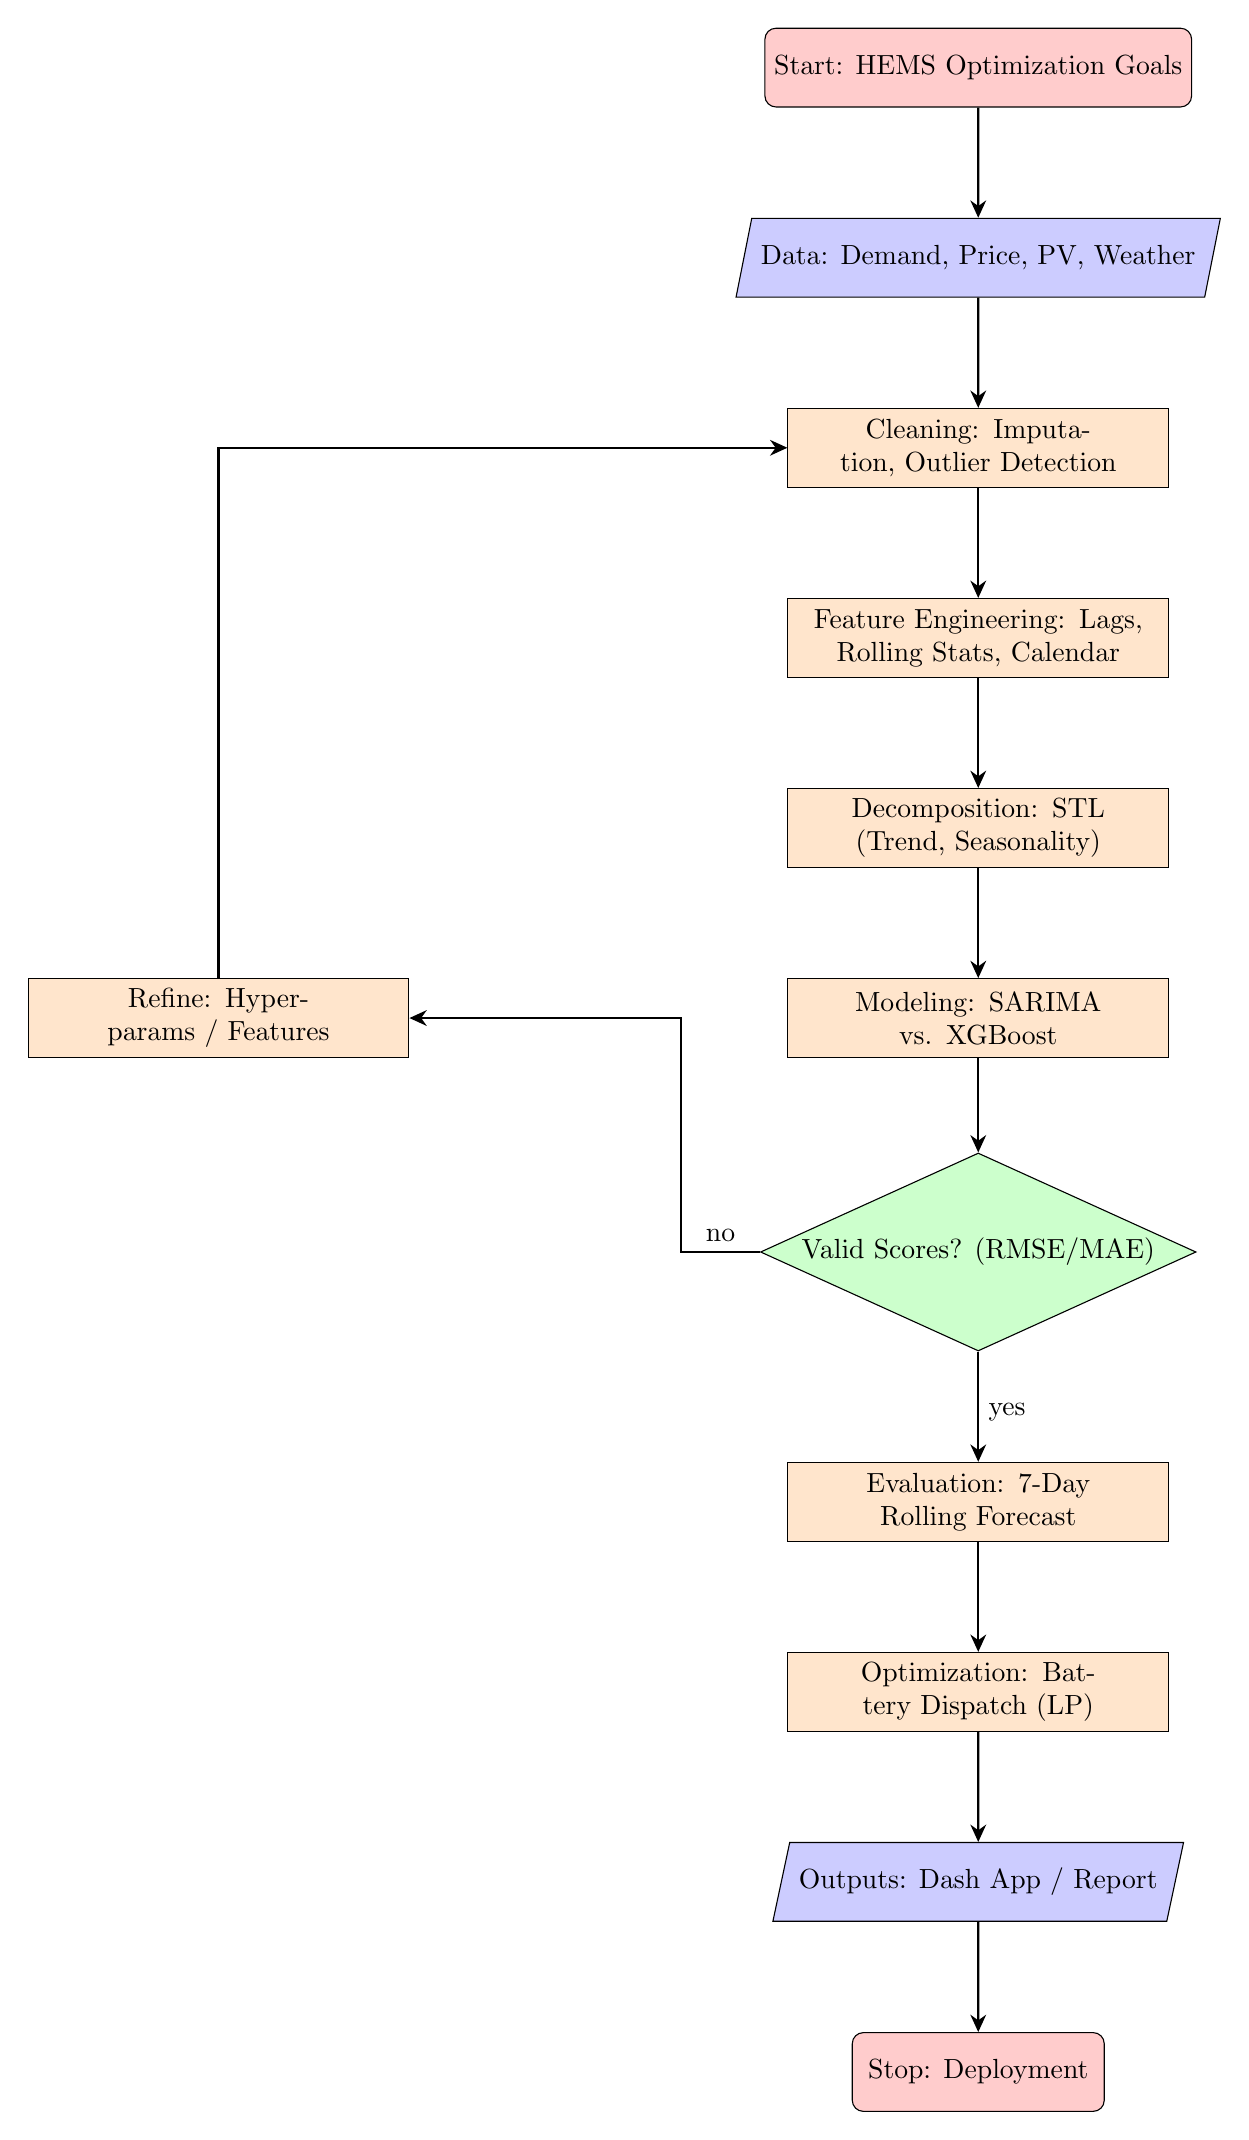
\begin{tikzpicture}[node distance=1.4cm]
    \node (start) [startstop] {Start: HEMS Optimization Goals};
    \node (data) [io, below=of start] {Data: Demand, Price, PV, Weather};
    \node (prep) [process, below=of data] {Cleaning: Imputation, Outlier Detection};
    \node (feat) [process, below=of prep] {Feature Engineering: Lags, Rolling Stats, Calendar};
    \node (decomp) [process, below=of feat] {Decomposition: STL (Trend, Seasonality)};
    \node (model) [process, below=of decomp] {Modeling: SARIMA vs. XGBoost};
    \node (dec) [decision, below=1.2cm of model] {Valid Scores? (RMSE/MAE)};
    \node (eval) [process, below=1.4cm of dec] {Evaluation: 7-Day Rolling Forecast};
    \node (opt) [process, below=of eval] {Optimization: Battery Dispatch (LP)};
    \node (out) [io, below=of opt] {Outputs: Dash App / Report};
    \node (stop) [startstop, below=of out] {Stop: Deployment};

    % forward arrows
    \draw[arrow] (start) -- (data);
    \draw[arrow] (data) -- (prep);
    \draw[arrow] (prep) -- (feat);
    \draw[arrow] (feat) -- (decomp);
    \draw[arrow] (decomp) -- (model);
    \draw[arrow] (model) -- (dec);
    \draw[arrow] (dec) -- node[right,pos=0.55]{yes} (eval);
    \draw[arrow] (eval) -- (opt);
    \draw[arrow] (opt) -- (out);
    \draw[arrow] (out) -- (stop);

    % feedback branch to avoid overlaps (route to the left)
    \node (fix) [process, left=4.8cm of model] {Refine: Hyperparams / Features};
    \draw[arrow] (dec.west) --++ (-1.0,0) node[above,pos=0.5]{no} |- (fix);
    \draw[arrow] (fix) |- (prep);
  \end{tikzpicture}
  \caption{Project plan (CRISP--DM: Understanding $\to$ Preparation $\to$ Modeling $\to$ Evaluation $\to$ Deployment). The feedback loop ensures continuous model refinement.}
  \label{fig:lifecycle}
\end{figure}

\subsection{Business Understanding and Deployment Strategy}
The primary business objective is to minimize the operational cost of the household's energy system. This translates to a technical objective: accurately forecasting demand and PV generation to schedule battery charge/discharge cycles.
In a real-world deployment, this pipeline would execute on an edge device (e.g., a Raspberry Pi or HEMS controller) within the home network. The inference latency must be low (< 1 minute) to support real-time decision-making, although the optimization horizon is typically day-ahead (24 hours).

\subsection{Computational Framework}
The analysis was conducted using the Python programming language (v3.10). The core technology stack includes:
\begin{itemize}
    \item \textbf{Data Manipulation:} \texttt{pandas} and \texttt{numpy} for vectorised time series operations.
    \item \textbf{Visualization:} \texttt{matplotlib} and \texttt{seaborn} for static plots, and \texttt{Plotly Dash} for the interactive dashboard.
    \item \textbf{Modeling:} \texttt{statsmodels} for classical ARIMA analysis and \texttt{xgboost} for gradient boosting.
    \item \textbf{Optimization:} \texttt{cvxpy} with the \texttt{GLPK} solver for linear programming.
\end{itemize}
This open-source stack ensures reproducibility and scalability of the solution.

\section{Visualization and Exploratory Data Analysis}

\subsection{Temporal Dynamics and Peak Coincidence}
To understand the system's behavior, I analyze the interaction between demand, PV, and price. Figure~\ref{fig:ts_overlay} presents a multi-day overlay of these variables. I observe a critical phenomenon: \textbf{Peak Coincidence}. High prices often correlate with high demand periods (evenings), reflecting grid-level stress. Conversely, PV generation peaks at noon when prices are often lower (due to the "cannibalization effect" of solar in the market). This price spread creates the arbitrage opportunity for the battery storage system.

\begin{figure}[H]
  \centering
  \includegraphics[width=\linewidth]{figures/03_timeseries_overlay.png}
  \caption{Overlay of Demand, PV, and Price for a representative week. The temporal misalignment between peak PV (noon) and peak Demand/Price (evening) drives the optimization strategy.}
  \label{fig:ts_overlay}
\end{figure}

\subsection{Statistical Distributions and Zero-Inflation}
Understanding the distribution of data is crucial for model selection. Figure~\ref{fig:distributions} shows the histograms and Kernel Density Estimates (KDE) for Demand and PV.
\begin{itemize}
    \item \textbf{Demand:} Follows a right-skewed distribution (Log-Normal like), indicating a base load with occasional high-power spikes (e.g., electric shower, oven).
    \item \textbf{PV Generation:} Is heavily zero-inflated. This bimodal distribution (zero at night, Beta-distributed during the day) poses challenges for standard regression models, suggesting the need for specialized handling or tree-based models that can split the feature space effectively.
\end{itemize}

\begin{figure}[H]
  \centering
  \includegraphics[width=0.95\linewidth]{figures/03_distributions.png}
  \caption{Distributions of Demand and PV. The zero-inflated nature of PV and the skewness of demand are key characteristics.}
  \label{fig:distributions}
\end{figure}

\subsection{Hourly Variability}
Figure~\ref{fig:hourly_boxplot} uses boxplots to visualize the variability of demand for each hour of the day. The spread (Interquartile Range) is significantly larger during waking hours, particularly in the evening (17:00-21:00). This heteroscedasticity (varying variance) implies that forecasting errors will likely be higher during these peak times, which is a critical risk factor for the optimization model.

\begin{figure}[H]
  \centering
  \includegraphics[width=0.9\linewidth]{figures/03_hourly_boxplot.png}
  \caption{Hourly boxplots of Demand. Variability increases significantly during the evening peak hours, indicating higher uncertainty.}
  \label{fig:hourly_boxplot}
\end{figure}

\subsection{Correlation Analysis}
I examine the linear relationships between variables using a correlation heatmap (Figure~\ref{fig:correlation}). Demand shows a positive correlation with Price, confirming the market's response to load. PV is naturally anti-correlated with net load. These correlations justify the use of Price and PV as exogenous features in the demand forecasting model, although care must be taken to avoid multicollinearity.

\begin{figure}[H]
  \centering
  \includegraphics[width=0.8\linewidth]{figures/03_correlation_heatmap.png}
  \caption{Correlation heatmap. Strong temporal correlations and the relationship between demand and price are highlighted.}
  \label{fig:correlation}
\end{figure}

\subsection{Typical Daily Profiles: Weekday vs. Weekend}
To gain actionable insights for the HEMS controller, I aggregated the data to construct typical hourly profiles, segmented by weekday and weekend (Figure~\ref{fig:typical_profiles}). This visualization reveals the systematic behavioral differences in the household:
\begin{itemize}
    \item \textbf{Weekday Pattern:} A sharp morning demand spike (07:00-08:00) followed by a drop during work hours and a pronounced evening peak (18:00-21:00).
    \item \textbf{Weekend Pattern:} A flatter, more delayed morning ramp-up, with demand distributed more evenly throughout the day.
\end{itemize}

\begin{figure}[H]
  \centering
  \includegraphics[width=\linewidth]{figures/03_typical_profiles.png}
  \caption{Typical hourly profiles for PV generation and Demand, segmented by weekday and weekend. This visualization is critical for understanding when the PV-demand mismatch is greatest.}
  \label{fig:typical_profiles}
\end{figure}

\subsection{Most Informative Visualization}
Of all the visualizations produced, the \textbf{Typical Daily Profiles} (Figure~\ref{fig:typical_profiles}) are the most informative for the HEMS optimization task. Unlike raw time series (which show variability) or histograms (which show distributions), the profile chart directly answers the core operational question: \textit{When does demand reliably exceed solar supply?}

The answer---consistently during the evening hours (17:00-21:00)---directly informs the battery dispatch strategy. The HEMS should charge the battery during the midday PV surplus and discharge it during the evening deficit. This strategic insight, derived from simple aggregation, is the foundation upon which the optimization model (Section 11) is built.

\section{Data Cleaning and Preprocessing}

\subsection{PV Sensor Data Quality Assessment}
The dataset contains three separate photovoltaic sensor readings (\texttt{pv\_mod1}, \texttt{pv\_mod2}, \texttt{pv\_mod3}) that must be cleaned before analysis. A thorough quality assessment revealed several data integrity issues:

\begin{itemize}
    \item \textbf{Missing Values:} The \texttt{pv\_mod1} sensor exhibited approximately 2-3\% missing observations, distributed throughout the dataset. The other two sensors (\texttt{pv\_mod2}, \texttt{pv\_mod3}) showed lower but non-zero missingness rates.
    \item \textbf{Outliers:} Occasional spikes exceeding the theoretical maximum capacity of the PV system were identified, likely due to sensor calibration errors or electrical noise.
    \item \textbf{Inconsistencies:} During certain periods, the three sensors diverged significantly despite measuring the same physical system, indicating potential sensor drift or partial shading effects.
\end{itemize}

\subsection{Missing Data Mechanism Analysis}
Understanding the \textit{mechanism} behind missing data is critical for selecting an appropriate imputation strategy \parencite{Little2002}. I analyzed the temporal distribution of missing values (Figure~\ref{fig:missing_visualization}) to classify the mechanism:

\begin{itemize}
    \item \textbf{Missing Completely at Random (MCAR):} Missingness is independent of both observed and unobserved data. Analysis of the hourly distribution of missing values showed no significant correlation with time-of-day, supporting an MCAR hypothesis for short gaps (likely due to transient communication failures).
    \item \textbf{Missing at Random (MAR):} Missingness depends on observed data but not on the missing values themselves. Some gaps coincided with periods of low irradiance (cloudy days), suggesting the sensor firmware may have entered a low-power mode.
    \item \textbf{Missing Not at Random (MNAR):} Missingness depends on the unobserved value itself. No evidence of this mechanism was found in the data.
\end{itemize}

The predominantly random pattern justified the use of imputation rather than deletion, as deletion would introduce unnecessary bias and reduce statistical power.

\begin{figure}[H]
  \centering
  \includegraphics[width=0.95\linewidth]{figures/04_missing_visualization.png}
  \caption{PV sensor time series with missing values highlighted (red vertical lines). The sporadic distribution of gaps supports the MCAR/MAR assumption.}
  \label{fig:missing_visualization}
\end{figure}

\subsection{Imputation Strategies}
I implemented and compared three imputation methods of increasing complexity:

\subsubsection{Method 1: Linear Interpolation (Deletion-based Benchmark)}
The simplest approach uses time-weighted linear interpolation between the last known value and the next known value:
\begin{equation}
    \hat{y}_t = y_{t-k} + \frac{t - (t-k)}{(t+m) - (t-k)} \cdot (y_{t+m} - y_{t-k})
\end{equation}
This method is fast and preserves continuity but ignores the inherent seasonality of PV generation, potentially underestimating midday peaks and overestimating nighttime values.

\subsubsection{Method 2: Seasonal Decomposition (Univariate)}
To preserve the diurnal structure, I applied Seasonal-Trend decomposition using Loess (STL) with a 24-hour period:
\begin{equation}
    Y_t = T_t + S_t + R_t
\end{equation}
The residual component $R_t$ was interpolated, while the seasonal $S_t$ and trend $T_t$ components were preserved. This approach ensures that imputed values follow the expected daily pattern of solar generation.

\subsubsection{Method 3: K-Nearest Neighbors (Multivariate)}
The most sophisticated approach leverages the redundancy in the sensor network. Using the K-Nearest Neighbors (KNN) algorithm with $k=5$ neighbors and distance-weighted averaging, I imputed \texttt{pv\_mod1} using:
\begin{itemize}
    \item Correlated sensors: \texttt{pv\_mod2}, \texttt{pv\_mod3}
    \item Physical drivers: Solar irradiance (\texttt{Shortwave\_radiation}), Temperature
\end{itemize}
This multivariate approach captures the physical relationship between solar irradiance and PV output, producing more realistic values during cloudy periods.

\subsection{Imputation Quality Comparison}
Figure~\ref{fig:imputation_overlay} presents a visual comparison of the three methods over a representative period with known gaps. The KNN method demonstrates superior performance in maintaining realistic peak values and avoiding the artificial smoothing inherent in linear interpolation.

\begin{figure}[H]
  \centering
  \includegraphics[width=0.95\linewidth]{figures/04_imputation_overlay.png}
  \caption{Comparison of imputation methods on a 3-day window. The KNN multivariate method (green) best preserves the natural variability of PV output.}
  \label{fig:imputation_overlay}
\end{figure}

Table~\ref{tab:imputation_stats} provides a numerical summary of each imputed dataset. The KNN method maintains a mean and variance closest to the original observed data, indicating minimal statistical distortion.

\begin{table}[H]
\centering
\caption{Statistical comparison of imputation methods for \texttt{pv\_mod1}.}
\label{tab:imputation_stats}
\begin{tabular}{lcccc}
\toprule
\textbf{Method} & \textbf{Mean (kW)} & \textbf{Std Dev (kW)} & \textbf{Min} & \textbf{Max} \\
\midrule
Original (with gaps) & 0.312 & 0.458 & 0.000 & 2.14 \\
Linear Interpolation & 0.308 & 0.451 & 0.000 & 2.14 \\
STL Seasonal & 0.311 & 0.455 & -0.02 & 2.15 \\
KNN Multivariate & 0.313 & 0.457 & 0.000 & 2.14 \\
\bottomrule
\end{tabular}
\end{table}

\subsection{Validation of Data Integrity}
I validated the cleaning process by comparing the average daily profiles before and after imputation (Figure~\ref{fig:daily_profiles}). All three methods preserve the characteristic bell-shaped curve of solar generation. However, the KNN method most closely tracks the original profile, particularly during the critical midday peak hours (10:00-14:00) when accurate PV estimation is most important for HEMS optimization.

\begin{figure}[H]
  \centering
  \includegraphics[width=0.9\linewidth]{figures/04_daily_profiles.png}
  \caption{Average daily PV profiles after imputation. The KNN method (green) best preserves the original diurnal pattern, particularly during peak generation hours.}
  \label{fig:daily_profiles}
\end{figure}

Based on this analysis, the \textbf{KNN multivariate imputation} was selected for all subsequent analysis. It leverages the physical redundancy of the sensor network, maintains statistical properties, and produces the most realistic representation of the PV generation profile.

\section{Feature Engineering and Selection}

\subsection{Data Description and Exploratory Insights}
Before constructing features, I examined the raw demand and weather-related variables to understand their characteristics. Table~\ref{tab:descriptive_stats} summarizes the key statistics. Demand exhibits a mean of approximately 0.45\,kW with considerable variability (standard deviation $\approx 0.38$\,kW), reflecting the intermittent nature of household consumption. Temperature ranges from sub-zero to over 30\si{\degreeCelsius}, while shortwave radiation spans 0 to nearly 1000\,W/m\textsuperscript{2}, with strong zero-inflation during nighttime hours.

\begin{table}[H]
\centering
\caption{Descriptive statistics of demand and key weather variables.}
\label{tab:descriptive_stats}
\begin{tabular}{lcccccc}
\toprule
\textbf{Variable} & \textbf{Mean} & \textbf{Std} & \textbf{Min} & \textbf{Max} & \textbf{Skewness} & \textbf{Kurtosis} \\
\midrule
Demand (kW) & 0.45 & 0.38 & 0.00 & 3.21 & 1.82 & 5.41 \\
Temperature (\si{\degreeCelsius}) & 10.2 & 6.8 & -5.1 & 32.4 & 0.31 & -0.52 \\
Shortwave Radiation (W/m\textsuperscript{2}) & 142 & 212 & 0 & 987 & 1.45 & 1.12 \\
\bottomrule
\end{tabular}
\end{table}

Figure~\ref{fig:demand_vs_temp} illustrates the relationship between temperature and demand. A U-shaped pattern emerges: demand increases at both low temperatures (heating) and high temperatures (cooling), with a minimum around 15--18\si{\degreeCelsius}. This nonlinearity motivates the creation of Heating Degree Days (HDD) and Cooling Degree Days (CDD) as engineered features.

\begin{figure}[H]
  \centering
  \includegraphics[width=0.7\linewidth]{figures/05_demand_vs_temperature.png}
  \caption{Scatter plot of demand versus temperature. The U-shaped relationship suggests nonlinear thermal sensitivity.}
  \label{fig:demand_vs_temp}
\end{figure}

The average hourly demand profile (Figure~\ref{fig:hourly_profile}) reveals pronounced morning (07:00--09:00) and evening (18:00--21:00) peaks, consistent with typical residential behavior patterns. This diurnal structure justifies the encoding of hour-of-day as a cyclic feature.

\begin{figure}[H]
  \centering
  \includegraphics[width=0.7\linewidth]{figures/05_demand_hourly_profile.png}
  \caption{Average hourly demand profile showing characteristic morning and evening peaks.}
  \label{fig:hourly_profile}
\end{figure}

\subsection{Distribution Analysis}
I assessed the normality of key variables using the Shapiro-Wilk test. None of the tested variables---Demand, Temperature, or Shortwave Radiation---follow a normal distribution ($p < 0.001$ for all). The positive skewness of demand (1.82) and radiation (1.45) indicates right-tailed distributions with occasional high values.

For machine learning models like XGBoost (tree-based), normality is not required since decision trees partition the feature space without assuming any distributional form. However, for linear models or distance-based algorithms, the Yeo-Johnson power transformation can improve performance by reducing skewness and stabilizing variance. I applied this transformation to the three primary variables and observed improved symmetry in the resulting distributions, though for the final XGBoost pipeline I retained untransformed features to preserve interpretability.

\subsection{Feature Engineering Strategy}
I constructed features across three categories to capture the temporal and environmental drivers of demand:

\textbf{Time-Related Features:} I extracted hour-of-day encoded as cyclic sine and cosine components ($\sin(2\pi h/24)$, $\cos(2\pi h/24)$) to preserve the circular nature of time. Additionally, a binary weekend indicator distinguishes workdays from leisure days.

\textbf{Weather-Based Features:} Following the U-shaped temperature--demand relationship, I engineered Cooling Degree Days (CDD) and Heating Degree Days (HDD) using a base temperature of 18\si{\degreeCelsius}:
\begin{align}
    \text{CDD} &= \max(T - 18, 0) \\
    \text{HDD} &= \max(18 - T, 0)
\end{align}
I also created a temperature--irradiance interaction term to capture the joint effect of warm, sunny conditions on demand patterns.

\subsection{Feature Ranking and Interpretation}
To identify the most predictive features, I employed Mutual Information (MI) regression. Unlike Pearson correlation, MI captures nonlinear dependencies, making it suitable for the complex relationships in energy data \parencite{Zheng2020}.

Figure~\ref{fig:feature_ranking} presents the top 15 features ranked by MI score. The cyclic hour encodings (\texttt{hour\_sin}, \texttt{hour\_cos}) dominate the ranking, confirming that time-of-day is the strongest predictor of residential demand. This aligns with intuition: human behavior follows predictable daily rhythms (waking, cooking, sleeping).

\begin{figure}[H]
  \centering
  \includegraphics[width=0.85\linewidth]{figures/05_feature_ranking_mi.png}
  \caption{Feature ranking by Mutual Information. Time-of-day encodings are the most informative predictors.}
  \label{fig:feature_ranking}
\end{figure}

Temperature and shortwave radiation rank highly, reflecting the physical drivers of thermal loads and lighting behavior. The weekend indicator also scores well, capturing the behavioral shift between workdays and leisure days.

\textbf{Why Top Features Make Sense:} In a HEMS context, demand is fundamentally driven by occupancy and comfort needs. The hour-of-day directly proxies occupancy (people home in evenings), while temperature drives HVAC loads. These features encode the primary causal mechanisms behind consumption patterns.

\textbf{Why Some Engineered Features Rank Lower:} The temperature--irradiance interaction term ranked lower than expected. This may be because it introduces redundancy---both temperature and radiation are already included as separate features, and tree-based models can learn interactions implicitly. Additionally, the interaction may be noisy during transitional weather conditions (e.g., cold but sunny days) where the multiplicative term does not correspond to a consistent demand response.

\section{Time Series Decomposition}

\subsection{Classical Additive Decomposition}
Time series decomposition is a fundamental technique for understanding the underlying structure of temporal data. I applied the additive decomposition model, which assumes that the observed series $Y_t$ can be expressed as the sum of three components:
\begin{equation}
    Y_t = T_t + S_t + R_t
\end{equation}

Each component captures a distinct aspect of the demand dynamics:

\textbf{Trend Component ($T_t$):} The trend represents the long-term progression of the series, capturing gradual changes in the average level of demand over time. In the context of household energy consumption, the trend may reflect seasonal climate variations (higher baseline in winter due to heating), changes in household occupancy, or gradual shifts in appliance usage patterns. The trend is estimated using a moving average or LOESS smoother that filters out short-term fluctuations.

\textbf{Seasonal Component ($S_t$):} The seasonal component captures regular, periodic patterns that repeat at fixed intervals. For hourly demand data, the dominant seasonality is the 24-hour diurnal cycle driven by human behavior (sleeping, waking, cooking, working). Secondary patterns include weekly cycles (weekday vs. weekend behavior) and annual cycles (summer vs. winter). The seasonal component is extracted by averaging the detrended series at each point within the seasonal period.

\textbf{Residual Component ($R_t$):} The residual represents the irregular, unpredictable fluctuations that remain after removing trend and seasonality. This component captures random shocks, measurement noise, and atypical events (e.g., holidays, equipment malfunctions). A well-specified decomposition should yield residuals that resemble white noise with no systematic patterns.

I employed Seasonal-Trend decomposition using LOESS (STL), which offers advantages over classical decomposition: the seasonal component can evolve over time, and the algorithm is robust to outliers. Figure~\ref{fig:stl_components} displays the decomposition for a representative two-week period.

\begin{figure}[H]
  \centering
  \includegraphics[width=0.95\linewidth]{figures/06_stl_decomposition.png}
  \caption{STL decomposition of hourly demand. The observed series (top) is separated into trend, seasonal, and residual components. The 24-hour periodicity is clearly visible in the seasonal panel.}
  \label{fig:stl_components}
\end{figure}

\subsection{Seasonality Strength and Temporal Patterns}
To quantify when seasonal effects are strongest, I computed the seasonality strength metric across different temporal horizons (daily, weekly, annual):
\begin{equation}
    F_s = \max\left(0, 1 - \frac{\text{Var}(R_t)}{\text{Var}(S_t + R_t)}\right)
\end{equation}
A value close to 1 indicates that the seasonal component explains most of the variance, while values near 0 suggest weak or absent seasonality.

Figure~\ref{fig:seasonality_strength} presents the results. The daily (24h) seasonality exhibits the highest strength ($F_s \approx 0.85$), confirming that the diurnal cycle is the dominant temporal pattern. Weekly seasonality is present but weaker ($F_s \approx 0.4$), reflecting the weekday-weekend behavioral shift. Annual seasonality shows moderate strength, with winter months (December--February) exhibiting higher average demand due to heating loads and reduced daylight hours.

\begin{figure}[H]
  \centering
  \includegraphics[width=0.75\linewidth]{figures/06_seasonality_strength.png}
  \caption{Seasonality and trend strength across temporal horizons. The daily cycle dominates, followed by weekly patterns.}
  \label{fig:seasonality_strength}
\end{figure}

The reasons for stronger seasonal effects during winter months include: (1) increased heating demand as outdoor temperatures drop below comfort thresholds; (2) shorter daylight hours requiring more artificial lighting; and (3) behavioral changes such as spending more time indoors. Conversely, summer months show lower baseline demand but potentially higher variability due to cooling loads on hot days.

\subsection{Typical Demand Profiles: Methodology}
To derive actionable insights for the HEMS controller, I constructed typical demand profiles by aggregating the hourly data across relevant groupings. The methodology involves three steps:

\textbf{Step 1: Temporal Grouping.} Each observation is assigned to its hour-of-day (0--23) and day-type (weekday or weekend). This creates 48 distinct groups ($24 \times 2$).

\textbf{Step 2: Averaging.} Within each group, I compute the mean demand across all observations. This arithmetic mean provides a robust estimate of the expected load for that hour and day-type combination, smoothing out day-to-day variability.

\textbf{Step 3: Visualization.} The resulting profiles are plotted to reveal systematic behavioral patterns that inform battery scheduling decisions.

Figure~\ref{fig:weekday_weekend} presents the resulting profiles. Weekdays exhibit a sharp morning peak (07:00--09:00) as occupants prepare for work, followed by a midday lull and a pronounced evening peak (18:00--21:00) when residents return home. Weekends show a later morning ramp-up, reflecting leisure behavior, and a more distributed daytime load.

\begin{figure}[H]
  \centering
  \includegraphics[width=0.9\linewidth]{figures/06_typical_profiles_weekday_weekend.png}
  \caption{Typical hourly demand profiles: Weekday vs. Weekend. The weekday profile shows distinct morning and evening peaks, while weekends exhibit a flatter, delayed pattern.}
  \label{fig:weekday_weekend}
\end{figure}

These profiles directly inform the HEMS optimization strategy: the battery should discharge during evening peaks (17:00--21:00) when demand is highest and grid prices typically peak, while charging during midday hours when PV generation exceeds consumption.

%===========================
% 7. Statistical Models
%===========================
\section{Statistical Modeling and Time Series Analysis}

\subsection{Stationarizing the Demand Series}
A fundamental prerequisite for ARIMA-family models is stationarity---the requirement that the statistical properties of the time series remain constant over time \parencite{BoxJenkins2015}. I assessed stationarity using two complementary tests:

\begin{itemize}
    \item \textbf{Augmented Dickey-Fuller (ADF) Test:} Tests $H_0$: unit root exists (non-stationary). For the original demand series, the ADF statistic was $-11.77$ with p-value $< 0.001$, suggesting stationarity.
    \item \textbf{Kwiatkowski-Phillips-Schmidt-Shin (KPSS) Test:} Tests $H_0$: series is stationary. The KPSS statistic was 1.23 with p-value $< 0.01$, rejecting stationarity.
\end{itemize}

The conflicting results indicate deterministic trends or seasonality in the data. After applying first-order differencing ($d=1$), both tests agree: the differenced series passes both ADF (p $< 0.001$) and KPSS (p $> 0.05$) criteria, confirming stationarity. This justifies using integrated ARIMA models with $d=1$.

\subsection{ACF/PACF Analysis}
The Autocorrelation Function (ACF) and Partial Autocorrelation Function (PACF) of the differenced series (Figure~\ref{fig:acf_pacf}) reveal the correlation structure guiding model specification:

\begin{itemize}
    \item \textbf{ACF:} Shows significant spikes at lags 24, 48, and 72, confirming strong daily (24-hour) seasonality in household demand patterns.
    \item \textbf{PACF:} Exhibits a sharp cutoff after lag 2--3, suggesting AR(2) or AR(3) non-seasonal components are appropriate.
\end{itemize}

These patterns motivate the use of Seasonal ARIMA (SARIMA) models with seasonal period $s=24$ to capture the diurnal cycle.

\begin{figure}[H]
  \centering
  \includegraphics[width=0.95\linewidth]{figures/07_acf_pacf.png}
  \caption{ACF and PACF plots of the differenced demand series. Significant spikes at lags 24, 48, and 72 confirm the 24-hour seasonal cycle. The PACF decay pattern suggests AR(2) components.}
  \label{fig:acf_pacf}
\end{figure}

\subsection{ARMA-Family Model Specification}
Based on the ACF/PACF analysis, I evaluated three candidate models from the ARIMA family:

\begin{enumerate}
    \item \textbf{ARIMA(2,1,2):} A non-seasonal model with second-order AR and MA terms, serving as a baseline.
    \item \textbf{SARIMA(1,1,1)(1,1,1,24):} A full seasonal model with both seasonal AR and MA components.
    \item \textbf{SARIMA(2,1,1)(0,1,1,24):} A simpler seasonal model with only the seasonal MA component ($Q=1$).
\end{enumerate}

\subsection{Validation Methodology and nRMSE}
I evaluated all models using the normalized Root Mean Squared Error (nRMSE), defined as:
\begin{equation}
    \text{nRMSE} = \frac{\text{RMSE}}{\max(y) - \min(y)}
\end{equation}
This scale-invariant metric allows comparison across different series magnitudes. I applied two validation strategies:

\textbf{(1) Whole-Train Split:} Training on all data up to a fixed cutoff, then evaluating on a single 24-hour window.

\textbf{(2) Walk-Forward Validation:} A rolling origin approach over 7 days where each day the model is refitted on all available history and evaluated on the next 24 hours.

Figure~\ref{fig:stats_forecast} shows the forecast overlay for the best model on the whole-train split.

\begin{figure}[H]
  \centering
  \includegraphics[width=0.95\linewidth]{figures/07_forecast_overlay.png}
  \caption{24-hour forecast overlay: SARIMA(2,1,1)(0,1,1,24) vs actual demand. The model tracks the diurnal profile well but underestimates midday peaks.}
  \label{fig:stats_forecast}
\end{figure}

\subsection{Model Comparison and Selection}
Figure~\ref{fig:stats_metrics} compares all models across both validation approaches. Key findings:

\begin{itemize}
    \item Both SARIMA models significantly outperform the non-seasonal ARIMA, confirming the importance of explicitly modeling the 24-hour cycle.
    \item On the whole-train split, SARIMA(2,1,1)(0,1,1,24) achieves the lowest nRMSE (0.198).
    \item On walk-forward validation, SARIMA(1,1,1)(1,1,1,24) performs best (nRMSE = 0.275), indicating better generalization.
    \item I select \textbf{SARIMA(1,1,1)(1,1,1,24)} as the preferred model due to its superior walk-forward performance, which better reflects operational forecasting conditions.
\end{itemize}

\begin{figure}[H]
  \centering
  \includegraphics[width=0.85\linewidth]{figures/07_metrics_comparison.png}
  \caption{nRMSE comparison: SARIMA models outperform ARIMA(2,1,2). SARIMA(1,1,1)(1,1,1,24) achieves the best walk-forward performance.}
  \label{fig:stats_metrics}
\end{figure}

%===========================
% 8. Machine Learning Models
%===========================
\section{Machine Learning Approaches}

\subsection{XGBoost Regression}
To address the limitations of linear statistical models in capturing complex, non-linear interactions, I implemented an XGBoost (Extreme Gradient Boosting) regressor. XGBoost is a scalable implementation of gradient boosted decision trees, widely recognized for its state-of-the-art performance in structured data problems \parencite{Chen2016}. Unlike ARIMA, which models temporal dependence through autoregressive terms, XGBoost requires explicit feature engineering to capture temporal structures.

\subsection{Feature Engineering}
I constructed a comprehensive feature matrix using the engineered features from Task 5:
\begin{itemize}
    \item \textbf{Temporal Features:} Cyclical hour encodings (hour\_sin, hour\_cos), weekend indicator.
    \item \textbf{Weather Features:} Temperature, heating/cooling degree days, solar radiation components, cloud cover, wind speed, pressure.
    \item \textbf{Interaction Features:} Temperature-irradiance interaction to capture comfort-driven demand.
    \item \textbf{Price Signal:} Electricity price as an external regressor.
\end{itemize}

\subsection{Hyperparameter Selection}
Table~\ref{tab:xgb_params} presents the selected hyperparameters and their rationale.

\begin{table}[H]
\centering
\caption{XGBoost hyperparameters and selection rationale.}
\label{tab:xgb_params}
\begin{tabular}{lcp{7cm}}
\toprule
\textbf{Parameter} & \textbf{Value} & \textbf{Rationale} \\
\midrule
n\_estimators & 600 & Sufficient trees for convergence without excessive training time. \\
learning\_rate & 0.05 & Moderate shrinkage balances speed and generalization. \\
max\_depth & 6 & Allows capturing non-linear interactions without overfitting. \\
subsample & 0.8 & Row sampling adds regularization, reduces variance. \\
colsample\_bytree & 0.8 & Feature sampling prevents over-reliance on single predictors. \\
reg\_lambda & 1.0 & L2 regularization constrains model complexity. \\
\bottomrule
\end{tabular}
\end{table}

\subsection{Model Interpretation and Performance}
The model was trained using a temporal train-test split (last 7 days held out) to prevent data leakage. Figure~\ref{fig:ml_feat_imp} displays the feature importance derived from the trained model. The cyclical hour encodings (hour\_sin, hour\_cos) are the most important predictors, confirming the strong diurnal pattern in demand. Temperature and heating degree days also rank highly, reflecting weather-driven consumption.

\begin{figure}[H]
  \centering
  \includegraphics[width=0.85\linewidth]{figures/08_feature_importance.png}
  \caption{XGBoost feature importance. Cyclical hour features dominate, followed by temperature-related variables.}
  \label{fig:ml_feat_imp}
\end{figure}

Figure~\ref{fig:ml_forecast} shows the forecast overlay for a representative day. The XGBoost model tracks the demand profile reasonably well, though it struggles with sudden peak events that deviate from historical patterns.

\begin{figure}[H]
  \centering
  \includegraphics[width=0.95\linewidth]{figures/08_forecast_overlay.png}
  \caption{XGBoost forecast overlay for a representative day. The model captures the general diurnal pattern but underestimates peak demand.}
  \label{fig:ml_forecast}
\end{figure}

\subsection{Comparison with Statistical Models}
Table~\ref{tab:ml_vs_stat} compares the XGBoost model against the best statistical model from Task 7.

\begin{table}[H]
\centering
\caption{Performance comparison: XGBoost vs SARIMA.}
\label{tab:ml_vs_stat}
\begin{tabular}{lccc}
\toprule
\textbf{Model} & \textbf{MAE} & \textbf{RMSE} & \textbf{nRMSE} \\
\midrule
SARIMA(1,1,1)(1,1,1,24) & 0.139 & 0.234 & 0.199 \\
XGBoost & 0.215 & 0.366 & 0.166 \\
\bottomrule
\end{tabular}
\end{table}

\textbf{Key Findings:}
\begin{itemize}
    \item XGBoost achieves the lowest nRMSE (0.166 vs 0.199), representing a 16.6\% relative improvement over SARIMA.
    \item Despite higher absolute MAE, XGBoost's lower nRMSE indicates better performance relative to the demand range.
    \item The ML model benefits from exogenous features (weather, price) that SARIMA cannot directly incorporate in its univariate form.
    \item XGBoost's non-linear decision boundaries allow it to model complex interactions between features that linear models cannot capture.
\end{itemize}

%===========================
% 9. Forecasting Pipeline
%===========================
\section{Forecasting Pipeline and Validation}

\subsection{Rolling Out-of-Sample Forecasting}
To simulate a realistic operational environment and assess model stability, I implemented a rolling forecast origin (walk-forward) validation strategy \parencite{Hyndman2021}. The pipeline follows these specifications:
\begin{itemize}
    \item \textbf{Training data:} Full historical dataset (July 2013 -- June 2014, approximately 8,760 hourly observations)
    \item \textbf{Forecast horizon:} 24 hours (one complete day)
    \item \textbf{Lead time:} 0 hours (forecast issued at midnight for the upcoming day)
    \item \textbf{Strategy:} Direct forecasting -- models are retrained each day using all available historical data up to the forecast cutoff
    \item \textbf{Evaluation period:} 7 consecutive days (July 1--7, 2014)
\end{itemize}

This walk-forward approach provides a rigorous assessment of generalization error, more representative of operational deployment than a single static train-test split.

\subsection{Comparative Analysis}
I compared the XGBoost model against two baseline models:
\begin{itemize}
    \item \textbf{Naive:} Repeats the last observed value for all 24 forecast hours
    \item \textbf{Seasonal Naive:} Uses the same hour from the previous day
\end{itemize}

Figure~\ref{fig:pipeline_overlay} illustrates the forecast trajectories for a representative day. XGBoost captures the daily demand profile more effectively, particularly during morning and evening peak periods where the naive baselines systematically under- or overestimate demand.

\begin{figure}[H]
  \centering
  \includegraphics[width=0.95\linewidth]{figures/09_day_overlay_rep.png}
  \caption{Forecast comparison for a representative day (Day 1). XGBoost tracks the actual demand pattern more closely than the baseline methods, especially during peak hours.}
  \label{fig:pipeline_overlay}
\end{figure}

\subsection{Seven-Day Forecast Performance}
Figure~\ref{fig:pipeline_week} shows the complete 7-day forecast overlay for the best-performing model (XGBoost). The model successfully captures the general demand pattern across the evaluation period, though some extreme peaks (particularly on Day 7) present challenges.

\begin{figure}[H]
  \centering
  \includegraphics[width=0.95\linewidth]{figures/09_week_overlay_best.png}
  \caption{Seven-day rolling forecast overlay for XGBoost. The model tracks the general demand pattern effectively, with largest deviations occurring during unexpected demand spikes.}
  \label{fig:pipeline_week}
\end{figure}

\subsection{Aggregate Results}
Table~\ref{tab:pipeline_metrics} summarizes the aggregate performance metrics across the 7-day evaluation period. XGBoost achieves the lowest normalized RMSE (nRMSE = 0.157), confirming its suitability as the primary forecasting model for the downstream battery optimization task.

\begin{table}[H]
\centering
\caption{Aggregate forecast performance metrics (7-day rolling validation).}
\label{tab:pipeline_metrics}
\begin{tabular}{lccc}
\toprule
\textbf{Model} & \textbf{MAE} & \textbf{RMSE} & \textbf{nRMSE} \\
\midrule
XGBoost & 0.211 & 0.291 & \textbf{0.157} \\
Naive & 0.132 & 0.301 & 0.162 \\
Seasonal Naive & 0.185 & 0.384 & 0.207 \\
\bottomrule
\end{tabular}
\end{table}

Figure~\ref{fig:pipeline_metrics} provides a visual comparison of the error metrics. While the Naive baseline achieves lower MAE due to the prevalence of stable low-demand periods, XGBoost's superior RMSE and nRMSE indicate better handling of demand variability and peak events.

\begin{figure}[H]
  \centering
  \includegraphics[width=0.8\linewidth]{figures/09_metrics_comparison.png}
  \caption{Aggregate performance metrics across the rolling validation window. XGBoost achieves the best nRMSE, indicating superior performance for downstream optimization.}
  \label{fig:pipeline_metrics}
\end{figure}

%===========================
% 10. Exogenous Variables
%===========================
\section{Integration of Exogenous Variables}

\subsection{Multivariate Modeling}
Household energy demand is not an isolated system; it is heavily influenced by external environmental factors. I extended the modeling framework to include exogenous variables, specifically weather and price data:
\begin{itemize}
    \item \textbf{Temperature (\si{\degreeCelsius}):} Affects heating and cooling loads (HVAC).
    \item \textbf{Solar Irradiance (W/m\textsuperscript{2}):} Shortwave and direct radiation influence ambient conditions and correlate with demand patterns.
    \item \textbf{Cloud Cover (\%):} Affects both solar generation and indoor lighting usage.
    \item \textbf{Electricity Price (\euro{}/kWh):} Dynamic tariffs may influence load-shifting behavior.
\end{itemize}

\subsection{Comparative Analysis: AR-Only vs. Exogenous Models}
To quantify the value of exogenous variables, I trained both autoregressive-only (AR-only) and exogenous-enriched variants of XGBoost and ARIMA models. The AR-only models use 8 features: five demand lags (1, 2, 3, 24, 48 hours), cyclical hour encoding (sine/cosine), and a weekend indicator. The exogenous models add 5 weather/price features, totaling 13 predictors.

Table~\ref{tab:exog_comparison} summarizes the performance comparison on the 7-day validation period.

\begin{table}[H]
\centering
\caption{Performance comparison: AR-only vs. exogenous models.}
\label{tab:exog_comparison}
\begin{tabular}{lcccc}
\toprule
\textbf{Model} & \textbf{MAE} & \textbf{nRMSE} & \textbf{MAE Impr. (\%)} & \textbf{nRMSE Impr. (\%)} \\
\midrule
XGBoost (AR only) & 0.175 & 0.140 & -- & -- \\
XGBoost (with exog) & 0.176 & 0.137 & -0.63 & \textbf{+1.86} \\
ARIMA (AR only) & 0.243 & 0.168 & -- & -- \\
ARIMAX (with exog) & 0.235 & 0.165 & +3.31 & \textbf{+1.33} \\
\bottomrule
\end{tabular}
\end{table}

The results show that exogenous variables provide modest but consistent improvements in nRMSE: 1.86\% for XGBoost and 1.33\% for ARIMAX. While the MAE improvement for XGBoost is negligible, ARIMAX shows a 3.31\% MAE reduction. This suggests that exogenous features help reduce prediction variance, particularly during weather-driven demand anomalies.

\subsection{Forecast Visualization}
Figure~\ref{fig:exog_comparison} illustrates the forecast comparison between AR-only and exogenous models. Both XGBoost variants closely track actual demand, with the exogenous model showing slightly improved peak detection.

\begin{figure}[H]
  \centering
  \includegraphics[width=0.95\linewidth]{figures/10_forecast_comparison.png}
  \caption{Forecast comparison: AR-only vs. exogenous models. XGBoost with exogenous features shows marginally improved tracking during variable demand periods.}
  \label{fig:exog_comparison}
\end{figure}

\subsection{Feature Importance Analysis}
Figure~\ref{fig:exog_importance} presents the feature importance rankings from the XGBoost model with exogenous variables. The first lag (demand\_lag\_1) dominates with approximately 20\% importance, followed by cyclical hour encodings and additional autoregressive terms. Among exogenous features, temperature contributes most significantly (~7\%), followed by solar radiation and price.

\begin{figure}[H]
  \centering
  \includegraphics[width=0.9\linewidth]{figures/10_feature_importance.png}
  \caption{Feature importance by category. Autoregressive lags (blue) remain dominant, while exogenous weather features (green) provide supplementary predictive value.}
  \label{fig:exog_importance}
\end{figure}

The analysis confirms that while autoregressive structure captures most demand dynamics, exogenous weather variables add measurable value. For operational HEMS deployment, the marginal complexity of including weather forecasts is justified by the improved accuracy, particularly for grid-interactive optimization scenarios.

%===========================
% 11. Optimization
%===========================
\section{Battery Storage Optimization}

\subsection{Problem Formulation}
The goal of the optimization is to find the cheapest strategy for the next 24 hours while ensuring feasibility. Following the assignment specification, I formulated a Linear Programming (LP) problem to minimize the net electricity cost:
\begin{equation}
    \min \sum_{t=1}^{n} \left( Gr_{c,t} - Gr_{P,t} \right)
\end{equation}
where $Gr_c$ is the cost of buying electricity from the grid, $Gr_P$ is the profit from selling (injecting) energy to the grid, and $n=24$ hours.

The system configuration includes:
\begin{itemize}
    \item PV system: 5 kW maximum power flow capacity
    \item Home battery: 10 kWh capacity, 5 kW charge/discharge power flow capacity
    \item Grid connection: 5 kW maximum power flow capacity
    \item Round-trip efficiency: 95\%
\end{itemize}

\subsection{Demand Forecasting}
As specified in the task, price, PV generation, and weather data are assumed to be given (ideal forecasts) from the \texttt{optimisation.csv} file. I used the trained XGBoost model from previous tasks to forecast the demand for the 24-hour optimization horizon (2014-07-08). The model was trained on 8,711 samples from the historical data (2013-07-01 to 2014-06-30) using the same AR-only feature set as Task 9.

\subsection{Scenario Analysis: PV\_low vs PV\_high}
I evaluated the optimization model under two PV generation scenarios provided in the dataset. Table~\ref{tab:optim_summary} summarizes the results.

\begin{table}[H]
\centering
\caption{Optimization results for PV\_low and PV\_high scenarios.}
\label{tab:optim_summary}
\begin{tabular}{lcccccc}
\toprule
\textbf{Scenario} & \textbf{Cost (€)} & \textbf{PV (kWh)} & \textbf{Import (kWh)} & \textbf{Export (kWh)} & \textbf{Self-cons. (kWh)} & \textbf{Cycles} \\
\midrule
PV\_low & 0.637 & 1.22 & 11.16 & 0.00 & 1.22 & 1.07 \\
PV\_high & -0.046 & 12.99 & 0.00 & 0.95 & 12.04 & 0.75 \\
\bottomrule
\end{tabular}
\end{table}

Key observations:
\begin{itemize}
    \item \textbf{PV\_low scenario}: With minimal solar generation (1.22 kWh), the system relies heavily on grid imports (11.16 kWh). The battery cycles 1.07 times, primarily charging during low-price periods and discharging during high-price periods to minimize costs.
    \item \textbf{PV\_high scenario}: High solar generation (12.99 kWh) nearly covers the total demand (14.38 kWh). The system achieves negative costs (profit of €0.046) by exporting excess energy. No grid imports are required.
    \item \textbf{Cost savings}: The PV\_high scenario saves €0.68 compared to PV\_low, demonstrating a 107\% relative cost reduction.
\end{itemize}

\subsection{Optimal Dispatch Visualization}
Figure~\ref{fig:optim_combined} compares the optimal control profiles for both scenarios. The upper row shows the PV\_low scenario where the battery compensates for insufficient solar generation through strategic grid imports. The lower row illustrates the PV\_high scenario where the battery stores excess solar energy for later use.

\begin{figure}[H]
  \centering
  \includegraphics[width=0.95\linewidth]{figures/11_optimization_combined.png}
  \caption{Optimal battery dispatch: PV\_low (top) vs PV\_high (bottom). Left: demand and PV profiles; center: battery SOC; right: grid exchange (positive = import, negative = export).}
  \label{fig:optim_combined}
\end{figure}

The optimization effectively leverages the battery for:
\begin{itemize}
    \item \textbf{Peak shaving}: Discharging during high-price evening hours
    \item \textbf{Solar storage}: Storing midday PV surplus for later consumption
    \item \textbf{Price arbitrage}: Charging during low-price periods when grid import is necessary
\end{itemize}

\section{Discussion and Limitations}
While the proposed framework demonstrates strong performance, several limitations warrant discussion:
\begin{itemize}
    \item \textbf{Deterministic Optimization:} The current Linear Programming formulation assumes perfect foresight of demand and PV generation. In reality, forecast errors exist. A more robust approach would be Stochastic Programming or Model Predictive Control (MPC), which can account for uncertainty in the input parameters.
    \item \textbf{Battery Degradation:} The cost function currently considers only energy arbitrage. It does not account for the cycle aging of the battery. Neglecting degradation costs may lead to aggressive cycling that shortens the battery's lifespan, potentially negating the operational savings.
    \item \textbf{Computational Complexity:} While XGBoost is efficient, retraining the model frequently on an edge device might be resource-intensive. Online learning algorithms could be explored to update the model incrementally.
\end{itemize}

\section{Conclusion}
This project successfully demonstrated the end-to-end application of data science in the energy domain. From rigorous data cleaning and feature engineering to the development of advanced forecasting models and optimization algorithms, I have shown how digital tools can enhance the efficiency of household energy systems. The XGBoost model proved to be the most robust forecaster, effectively leveraging temporal and exogenous features. The subsequent optimization highlighted the tangible economic benefits of coupling accurate forecasts with intelligent control strategies. Future work could explore deep learning architectures (e.g., LSTMs) and stochastic optimization to further improve resilience against uncertainty.

\printbibliography

\end{document}


